% Compile with pdfLaTeX and BibTeX (or latexmk -pdf).
\documentclass[12pt]{article}
\usepackage[T1]{fontenc}
\usepackage{lmodern}
\usepackage{amsmath,amssymb,graphicx,booktabs,tabularx,array}
\usepackage{xcolor,enumitem,float}
\usepackage{algorithm,algorithmic,multirow}
\usepackage[section]{placeins}
\usepackage[authoryear,square]{natbib}
\usepackage[hidelinks]{hyperref}
\usepackage{xurl}
\usepackage{microtype}
\setcounter{topnumber}{3}
\setcounter{bottomnumber}{2}
\setcounter{totalnumber}{5}
\renewcommand{\topfraction}{.92}
\renewcommand{\bottomfraction}{.85}
\renewcommand{\textfraction}{.08}
\renewcommand{\floatpagefraction}{.85}
\setlength{\textfloatsep}{14pt plus 2pt minus 2pt}
\setlength{\floatsep}{12pt plus 2pt minus 2pt}
\setlength{\emergencystretch}{2em}
\newif\ifmarked
\ifdefined\MarkedVersion\markedtrue\else\markedfalse\fi
\definecolor{revisionblue}{RGB}{24,70,140}
\newenvironment{revised}{\ifmarked\color{revisionblue}\fi}{}
\newcommand{\rev}[1]{{\ifmarked\color{revisionblue}\fi#1}}
\newcommand{\paperfigure}[4]{\begin{figure}[!htbp]\centering
  \includegraphics[width=#4\linewidth]{figures/#1.png}
  \caption{#2}\label{#3}\end{figure}}
% AUTO-GENERATED from actual ten-seed results.
\newcommand{\ExtSimpleBFone}{0.560}
\newcommand{\ExtSimpleBAP}{0.491}
\newcommand{\ExtMultiFone}{0.497}
\newcommand{\ExtMultiReview}{0.365}


\begin{document}
\begin{center}
{\bf Anomaly Detection Algorithm for Enhanced Fraud
Identification in the Insurance Sector}\\
{\sc Mehrab Atighi$^{a}$, Sayed Jamal Mirkamali$^{b}$,
Amir T. Payandeh Najafabadi$^{a,}$\footnote{amirtpayandeh@sbu.ac.ir}}\\
a Department of Actuarial Science, Faculty of Mathematical
Sciences, Shahid Beheshti University,
Evin, 1983969411, Tehran, Iran.\\
b Department of Mathematics, Faculty of Science, Arak University,
3848177584, Arak, Iran.\\
\today




\end{center}
\ifmarked
\noindent\colorbox{yellow!25}{\parbox{\dimexpr\linewidth-2\fboxsep}{
\textbf{Revision guide.} The original five-section organization and Algorithms
1--3 and the original workflow images are retained. Blue text marks additions and substantive corrections;
minor language and citation edits are not individually colored. Empirical
tables and plots replace the earlier exports. The change map identifies
removed claims and the source diff records textual changes.}}\medskip
\fi
\begin{abstract}
\begin{revised}
Insurance-fraud screening requires effective detection under class
imbalance and limited verification resources. Sequential Anomaly Detection
(SAD) uses an anomaly ensemble to select claims for review, then trains
eight supervised learners on verified records and updates them across
successive batches. Three architectures differ in their initial screening:
Simple-A uses nine anomaly detectors, Simple-B adds an entropy vote, and
Multilayer applies entropy after anomaly consensus. We evaluate these
architectures using ten repeated stratified random splits of Carclaims
(15,420 records; 5.99\% fraud) and Insurance Claims (1,000 records;
24.70\% fraud). Recorded outcomes simulate verification after case selection,
including random audits of non-alerted claims. At fixed voting thresholds
$(3,4)$, Simple-B achieves mean fraud F1 \ExtSimpleBFone{} and average
precision \ExtSimpleBAP{} on the second benchmark. Multilayer achieves F1
\ExtMultiFone{} at a review fraction of \ExtMultiReview{}. A frozen-model
ablation, ten classifiers trained under a common acquisition policy, and
a stricter threshold setting examine the effects on detection and workload.
The findings support assessment of both outcomes when selecting a review
policy; they do not establish universal architectural superiority or
prospective generalizability to an independent insurer.
\end{revised}
\end{abstract}
\noindent\textbf{Keywords:} insurance fraud; sequential updating; anomaly
detection; entropy; verification workload; class imbalance.
\par\noindent{\bf MSC2010}: {62D05, 62F10, 62N01, 65C05.}
\section{Introduction}\label{sec:introduction}
Insurance fraud creates financial losses and places demands on claims
investigation. Insurers must identify suspicious claims while allocating
limited review resources \citep{A61,Bolton2002}. This task is difficult
because legitimate claims are heterogeneous and unusual observations are
not necessarily fraudulent.

Machine-learning approaches address this problem through supervised
classification, unsupervised screening, or combinations of the two
\citep{Ngai2011,West2016,Schrijver2024}. Their practical value depends on
both detection performance and the number of claims requiring verification.
Selective investigation also determines which labels become available
for subsequent training.

Sequential Anomaly Detection (SAD) connects initial anomaly screening to
verification and repeated supervised learning. The framework is intended
to support a choice between detection performance and review workload.
We examine this choice through the simple and multilayered SAD structures.

\begin{revised}
The contribution lies in the organization and evaluation of established
components within a verification-driven workflow. Its \emph{sequential}
mechanism incorporates verified records from one batch into training before
the ensemble screens the next batch. Its \emph{multilayer} mechanism
applies an entropy filter to the candidates selected by anomaly-detector
consensus. Updating changes the information available for later prediction;
layering changes which initial cases reach verification. Simple-A,
Simple-B and Multilayer retain the original architectural alternatives:
entropy is absent, contributes a flat vote, or forms a second screening
layer, respectively.

The evaluation compares these three architectures, introduces a frozen-model
control for sequential updating, and applies the same prescribed protocol
to two benchmark datasets. Additional classifiers include an imbalance-aware
forest and a recent fraud-motivated boosting approach. The experiments
explicitly account for review workload and designate fraud as the positive
class. Recorded outcomes simulate expert feedback and are revealed to the
learner only after review selection. SAD uses fixed acquisition rules;
the comparison with reinforcement learning therefore concerns workflow
design rather than a learned reward-maximizing policy.
\end{revised}

Section \ref{SC:LR} positions SAD within the fraud-detection literature.
Section \ref{SC:METHOD} defines its components and update rules;
Section \ref{SC:RESULT} reports the benchmark experiments.
Section \ref{SC:CONCLUSION} discusses the findings and their limitations.

\section{LITERATURE REVIEW}\label{SC:LR}\label{sec:literature}
\begin{revised}
The literature is grouped below by the information used for learning and
the role of verification in each approach.
Early statistical and data-mining reviews distinguish label-based detection
from anomaly screening \citep{Bolton2002,Ngai2011}; broader financial-fraud
reviews describe their continuing complementarity \citep{West2016,A61}.
The systematic review of \citet{Schrijver2024} describes the prominence of
supervised learning and oversampling in automobile-insurance fraud studies,
as well as limitations in public data availability.

\subsection{Supervised approaches}
Supervised models use previously investigated claims to estimate a decision
boundary or ranking. Regression, support-vector machines, forests, boosting,
and neural networks are common choices \citep{A80,A61}. Insurance-specific
work includes optimized boosting and interpretable assessment
\citep{Ding2025}, practical model-selection guidance
\citep{BanulescuRadu2024}, and imbalance and missing-value handling
\citep{Khalil2024}. These methods can exploit claim attributes effectively
when their training labels are sufficiently representative. Direct comparisons
of supervised and unsupervised insurance models are also reported by
\citet{Debener2023}. Selective
historical investigation, however, can bias which examples are labeled.

In \emph{Annals of Data Science}, \citet{Kamalov2023} examine feature selection
under imbalance and propose a minority-sensitive criterion. Their work
motivates explicit attention to fraud-class metrics here; we do not equate
our unsupervised Gini screen with their supervised selection algorithm.

\subsection{Unsupervised approaches}
Anomaly methods rank observations according to deviations from a fitted
notion of normality. Auto-insurance applications include spectral ranking
\citep{Nian2016} and unsupervised deep learning \citep{Gomes2021}.
Such approaches can propose cases before reliable labels exist, but unusual
observations need not be fraudulent. Clustering methods also depend on
representation and dissimilarity choices, as reviewed by
\citet{XuTian2015} in \emph{Annals of Data Science}. This supports using
heterogeneous signals while retaining verification of their interpretation.

\subsection{Reinforcement-learning-based approaches}
When verification is costly, a learned policy can decide which observations
justify acquiring an outcome. In the framework studied by \citet{A73},
reinforcement learning guides this information-acquisition decision for
outlier detection. Actions are evaluated through a reward signal. SAD instead uses fixed voting
thresholds and a random audit fraction; it has no learned reward-maximizing
query policy. Its sequential component is retraining after each reviewed
batch, which can be tested against a frozen model.

\subsection{Hybrid architectures}
Hybrid approaches combine representations or learners, while graph methods
use relationships among claims, people, or entities \citep{Vorobyev2024}.
PSO-XGBoost is a recent insurance-specific example of optimization combined
with boosting \citep{Ding2025}. \citet{Hassani2020}, in \emph{Annals of Data
Science}, review deep-learning applications in banking, providing broader
financial-domain context. That review is contextual evidence, not a direct
insurance-fraud performance comparator.

\subsection{Research gap and comparator scope}
SAD addresses the connection between candidate generation, review, and
iterative learning. It does not replace the need for representative labels
or resolve all challenges in recent deep or graph-based systems.
Table \ref{tab:positioning} distinguishes these roles. The numerical
experiments include an explicitly adapted PSO-XGBoost comparator and balanced
random forests in addition to eight component classifiers. We do not
attribute our adapted implementation's numbers to the original publication.

\begin{table}[tbp]\centering\footnotesize
\caption{Comparative positioning by learning and acquisition mechanism.}
\label{tab:positioning}
\begin{tabularx}{\linewidth}{>{\raggedright\arraybackslash}p{2.5cm}*{3}{>{\raggedright\arraybackslash}X}}
\toprule
Family & Representative source & Strength & Boundary relevant to SAD\\\midrule
Supervised & Ding et al.; Banulescu-Radu and Yankol-Schalck & Direct label-based discrimination & Needs representative verified labels\\
Unsupervised & Nian et al.; Gomes et al. & Initial screening without outcomes & Anomaly is not confirmed fraud\\
Reinforcement learning & Nijhuis and van Lelyveld & Values costly information & Requires a query/reward design\\
Hybrid/graph & Vorobyev; Ding et al. & Relational or optimized predictive signals & May require links or additional tuning\\
SAD & This study & Explicit review and batch update workflow & Retrospective simulation; policy-dependent labels\\
\bottomrule
\end{tabularx}
\end{table}

\begin{table}[tbp]\centering\footnotesize
\caption{Mechanisms of recent counterparts compared with SAD.
Design comparison does not imply numerical reproduction.}
\label{tab:mechanisms}
\begin{tabularx}{\linewidth}{>{\raggedright\arraybackslash}p{2.8cm}*{3}{>{\raggedright\arraybackslash}X}}\toprule
Method & Main mechanism & Relation to sequential review & Relation to multilayer SAD\\\midrule
PSO-XGBoost \citep{Ding2025} & Optimized boosted trees & Search tunes parameters; it does not implement batch review & No post-consensus entropy gate specified\\
Unsupervised deep learning \citep{Gomes2021} & Learned anomaly representation & Does not by itself define SAD's verified-label accumulation & Different initial scoring mechanism\\
Costly-verification RL \citep{A73} & Reward-driven information acquisition & Learns an acquisition policy; SAD uses fixed rules & SAD's entropy gate is not a reward policy\\
Claims graph features \citep{Vorobyev2024} & Relational feature construction & Requires links beyond independent claim attributes & Adds relational information rather than SAD's entropy gate\\
SAD, this study & Anomaly votes, verification, supervised votes & Retrains once after each reviewed batch & Applies candidate-local EAD after initial consensus\\
\bottomrule\end{tabularx}\end{table}
\end{revised}

\section{METHODOLOGY}\label{SC:METHOD}\label{sec:methods}
SAD combines predictor preprocessing, anomaly screening, supervised
classification and batch-wise model updating. The following subsections
specify these components, their integration and the evaluation measures.

\subsection{PRE PROCESSING}\label{SSC:PreProcessing}
Dimensionality reduction decreases the number of input variables while
retaining useful characteristics of the data. In this research, the
preprocessing step uses feature screening through a Gini criterion for
categorical variables and a near-zero-variance criterion for numerical
variables \citep{Hastie2009,Kuhn2008}.

\subsubsection*{Dimension Reduction}
\textbf{Gini Index:} For a categorical predictor with category frequencies
$p_r$, the Gini impurity is
\[
Gini=1-\sum_{r=1}^{R}p_r^2.
\]
It is zero for a constant feature and increases as the observations are
distributed more evenly across categories. We retain predictors with
$g_L<Gini<g_U$, where $g_L=0.1$ and $g_U=0.9$.
\rev{This marginal variability screen does not measure association with fraud;
it can discard informative high-cardinality features.}

\textbf{Near Zero Variance:} Numerical predictors are removed if constant,
or if their most-common to second-most-common value frequency ratio exceeds
19 and their percentage of unique values is at most 10\%, following the
near-zero-variance screening convention \citep{Kuhn2008}.

\rev{To prevent information from later evaluation batches entering fitted
preprocessing, partitioning precedes feature screening. The screen, missing
value handling, scaling and categorical encoding are fitted using $D_1$
predictors only, as made explicit in Algorithm \ref{algo:preprocessing}.}
\begin{algorithm}[htbp]
\footnotesize
\caption{PreProcessing Algorithm}\label{algo:preprocessing}
\begin{algorithmic}[1]
\REQUIRE Dataset $D$; partition fractions $p_1,\ldots,p_m$; Gini bounds $g_L,g_U$
\ENSURE Partitions $D_1,\ldots,D_m$ and fixed predictor transformations
\STATE \rev{Withhold outcomes from predictors; retain original row identities.}
\STATE \rev{Partition records with sizes proportional to $p_1,\ldots,p_m$.}
\STATE \rev{On $D_1$ only, remove categorical predictors outside $(g_L,g_U)$ in Gini impurity.}
\STATE \rev{On $D_1$ only, remove numerical predictors satisfying near-zero variance.}
\STATE \rev{Fit imputation, scaling and encoding on retained $D_1$ predictors.}
\STATE \rev{Apply those fixed transformations to every partition $D_j$.}
\end{algorithmic}
\end{algorithm}


\begin{revised}
Policy identifiers, postal identifiers and incident addresses are excluded.
Near-unique categorical fields are also excluded. The two date fields in
Insurance Claims are expanded into year, month and weekday; this does not
make the experimental split chronological. The marker \texttt{?} is treated
as missing. Numerical medians and categorical modes provide imputation;
scaling and one-hot encoding use $D_1$ parameters and levels, with unseen
categories mapped to zero indicators. Outcomes are removed by name before
any detector or transformation is fitted, and row identities are preserved.
\end{revised}

\subsubsection*{Balancing}
\textbf{Resampling structure:} We use the Synthetic Minority Over-sampling
Technique (SMOTE) to address class imbalance during supervised training
\citep{Chawla2002,He2009}. SMOTE constructs additional minority-class
training vectors along line segments joining a minority observation to a
nearby observation from the same class.
\rev{In the revised experiments, SMOTE is applied only to accumulated
verified training records, never to future evaluation observations.
The neighbor count is at most five and is reduced for small minority sets.
One minority observation invokes random oversampling; a single-class set
raises an error. SMOTE operates on encoded features, so synthetic one-hot
values may be fractional. These are training vectors, not synthetic policies.
Previously generated synthetic records are not accumulated across rounds.}

\subsection*{Structure}
The two SAD workflows are illustrated below.
Figure \ref{figai1} connects preprocessing and data partitioning to
initial anomaly screening, verification and supervised learning. In subsequent iterations, the trained
models identify potential fraud in the next subset, followed by expert
confirmation and model updating.
Figure \ref{figai2} shows the multilayered structure, where EAD is applied
to the result of anomaly consensus before expert verification.
\rev{Figures 1 and 2 provide conceptual overviews of the retained workflows.
Algorithms 1--3 specify their implementation: preprocessing is fitted on $D_1$ after partitioning; expert review
includes alerts and a random sample of non-alerts; both fraud and genuine
verified records enter training (the diagram label ``Frauds'' is shorthand
for the reviewed records); and no model is retrained after the last evaluation
batch. The terminal trained model in the conceptual diagrams is relevant only
if further batches will arrive. Simple-A uses nine initial detector votes;
Simple-B adds entropy as a tenth vote. In Multilayer, EAD gates the initial
candidate subset before verification.}

\begin{figure}[!htbp]\centering
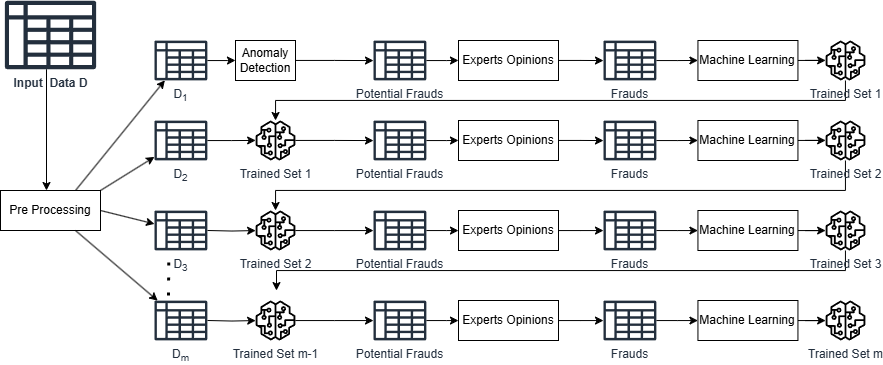
\includegraphics[width=\textwidth]{figures/simple.png}
\caption{Simple SAD workflow: initial screening, verification and model updating
across successive batches.}\label{figai1}
\medskip
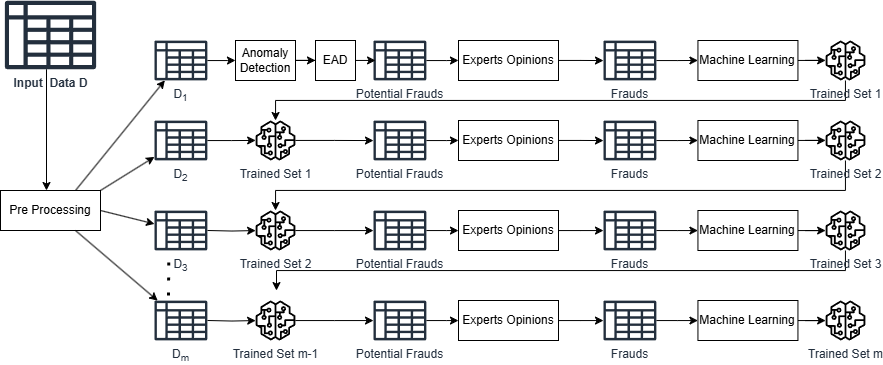
\includegraphics[width=\textwidth]{figures/Multilayered.png}
\caption{Multilayered SAD workflow, with entropy screening between initial
anomaly consensus and verification.}\label{figai2}
\end{figure}

\subsection*{ANOMALY DETECTION}\label{SSC:AD}
Before verified labels become available, the initial ensemble screens
claims for departures from empirical feature patterns. An anomaly flag
indicates a case for review, not a confirmed fraud \citep{Chandola2009}.
The nine retained detectors are specified below.

\textbf{Box Plot:} Observations outside
$[Q_1-1.5IQR,Q_3+1.5IQR]$, where $IQR=Q_3-Q_1$, are flagged
using the boxplot rule. The rule is applied separately to retained numerical
features, and the union of flagged records supplies one detector vote.

\textbf{Percentile structure:} Percentiles divide an empirical distribution
according to its cumulative frequency. Values below the fifth percentile
or above the ninety-fifth percentile are flagged in each numerical feature;
the union provides one vote.

\textbf{Z-score structure:} The Z score compares an observation with a
feature's mean and standard deviation. The prescribed rule flags
$|Z|>3$. Its interpretation depends on the feature distribution.

\textbf{Hampel filter structure:} Robust location and scale reduce the
influence of extreme values \citep{Hampel1974}. Here the batch-wise rule
flags a numerical value when its distance from the median exceeds
$3\times1.4826\times MAD$. It is not a sliding temporal filter.

\textbf{Grubbs test structure:} Grubbs' test compares an extreme standardized
deviation with a sample-size-dependent critical value under a normality
assumption \citep{Grubbs1969}. We use the two-sided critical threshold at
$\alpha=0.05$ as a screening rule. This is not an iterative multiple-outlier
hypothesis-testing procedure.

\textbf{KNN structure:} Distance-based outlier methods assess how far an
observation lies from neighboring observations \citep{Ramaswamy2000}.
The implemented score is the mean distance to five neighbors in standardized
numerical space; the top 20\% are flagged. This averaging is an implementation
choice, rather than an exact reproduction of the cited $k$th-distance rule.

\textbf{Local outlier factor (LOF) structure:} LOF quantifies how sparse an observation's neighborhood is relative
to the neighborhoods of nearby observations \citep{Breunig2000}.
The implementation uses 20 neighbors and a contamination setting of 0.15.

\textbf{Isolation forest structure:} Isolation Forest constructs randomized
partition trees and scores observations using their isolation paths
\citep{Liu2008}. We use 200 trees, subsamples of at most 256 records and
contamination 0.10 on the encoded predictor matrix.

\textbf{K Modes structure:} K-Modes extends centroid-based clustering to
categorical observations using category matching and modal representatives
\citep{Huang1998}. We use up to 30 clusters, one Huang initialization and
20 iterations, flagging the five smallest nonempty clusters. Small cluster
membership is a screening heuristic, not evidence of fraud by itself.

\textbf{Entropy Anomaly Detection (EAD):} The information content of a
categorical feature is measured by Shannon entropy \citep{Shannon1948}.
The original removal-based EAD idea compares the entropy of a working
dataset with its entropy after one observation is removed.
\begin{revised}
For subset $S$ and predictor $\ell$, let
$H_\ell(S)=-\sum_r p_{\ell r}\log_2p_{\ell r}$.
The exact implemented score is
\begin{equation}\label{eq:entropy}
Gain(x_i;S)=\frac{1}{p}\sum_{\ell=1}^{p}
\{H_\ell(S)-H_\ell(S\setminus\{x_i\})\}.
\end{equation}
Numerical variables use up to ten quantile bins fitted on $S$; those bins
remain fixed during leave-one-out calculation. Frequency counts permit
exact scores without rebuilding the dataset for every removal. The highest
20\% of scores form the entropy shortlist. Simple-B computes EAD on $D_1$;
Multilayer computes it on the anomaly-consensus subset $Y_1$.
\end{revised}

\textbf{Threshold limits:} The anomaly threshold $T_{AD}$ specifies the
minimum number of positive detector votes required to flag an observation.
A record is flagged once its positive-vote count reaches $T_{AD}$.
The threshold operates on detector consensus.

\subsection{MACHINE LEARNING}\label{SSC:ML}
Following anomaly detection, expert opinions supply training labels for
supervised learning. The ensemble includes the following eight model
families already used in the thesis implementation.

\textbf{LR models:} Logistic regression estimates a binary outcome
probability from the input features \citep{Hastie2009}.

\textbf{SVM models:} A support-vector classifier constructs a separating
hyperplane; kernel extensions can model nonlinear boundaries
\citep{Cortes1995}. The present ensemble uses a linear kernel.

\textbf{XGB models:} XGBoost builds an additive ensemble of decision trees
with regularized gradient boosting \citep{Chen2016}.

\textbf{RF models:} Random forests combine trees trained with randomized
observations and feature selections; their collective predictions form an
ensemble estimate \citep{Breiman2001}.

\textbf{NB models:} Naive Bayes combines class-conditional feature models
under a conditional-independence assumption \citep{Domingos1997}. The
implementation uses Gaussian feature likelihoods.

\textbf{KNN models:} Nearest-neighbor classification uses labeled examples
close to the observation being classified \citep{Cover1967}. This supervised
component is distinct from the initial KNN outlier detector.

\textbf{AdaBoost models:} AdaBoost combines weak learners through
successive reweighting of training observations \citep{Freund1997}.

\textbf{ANN models:} Artificial neural networks learn weights between
interconnected layers to model relationships between predictors and
outcomes \citep{Rumelhart1986}. We use one hidden layer.

\begin{revised}
\begin{table}[tbp]\centering\small
\caption{Fixed specifications of the original eight supervised model families.}
\label{tab:learners}
\begin{tabularx}{\linewidth}{p{2.0cm}X}\toprule
Model & Specification\\\midrule
LR & L2 logistic regression; liblinear; $C=1$; 1,000 iterations\\
SVM & Linear kernel; $C=1$; training-only probability estimation\\
XGBoost & 120 trees; depth 4; learning rate .05; row/column subsampling .8\\
RF & 200 trees; minimum leaf size 2\\
NB & Gaussian conditional feature model\\
KNN & Five neighbors; distance weighting\\
AdaBoost & 100 decision stumps; learning rate .5\\
ANN & 32 hidden units; L2 penalty $10^{-4}$; at most 200 iterations;
early stopping with 15\% internal validation\\
\bottomrule\end{tabularx}\end{table}
\end{revised}

\textbf{Threshold limit:} The supervised threshold $T_{ML}$ specifies the
minimum number of positive model votes for an alert.
\rev{For learner $k$, $V_k(x)=\mathbb{1}\{\hat p_k(x)\geq0.5\}$, and
$\hat y(x)=\mathbb{1}\{\sum_{k=1}^{M}V_k(x)\geq T_{ML}\}$.
The mean score $M^{-1}\sum_k\hat p_k(x)$ is used for ranking metrics.
After oversampling, that score need not be a calibrated population fraud
probability.}

\subsection{Sequential Anomaly Detection (SAD)}\label{SSC:SAD}
In the following, we describe two structures using the partitions returned
by Algorithm \ref{algo:preprocessing}. The inputs include the anomaly
detector set $AD\ SET$, the supervised model set $ML\ SET$, their sizes
$N$ and $M$, vote thresholds $T_{AD}$ and $T_{ML}$, expert opinions and the
non-alert sampling percentage $PN$.

\begin{revised}
Throughout the algorithms, ``potential normal'' means \emph{not alerted},
not verified genuine. In batch $j$, $F_j$ is the alert set and $G_j$ is a
random sample of $\lceil(PN/100)|D_j\setminus F_j|\rceil$ non-alerts.
Both sets are submitted for verification before their labels are available
to the learning algorithm. $E_j$ denotes these newly verified records,
$L_j=\bigcup_{r\leq j}E_r$ the accumulated real training records, and
$E'_j=SMOTE(L_j)$ the current balanced training set. In the experiments,
$PN=10$. Stored outcomes simulate expert opinions; no actual expert
investigation was conducted in this retrospective evaluation.
\end{revised}

\subsubsection*{Simple structure of the SAD algorithm}\label{sec4_2}
The anomaly detection process starts with unlabeled data from the first
partition. Every detector supplies a normal (0) or anomalous (1) vote for
each observation. The total $U_{Total}$ is compared with $T_{AD}$ to identify
potential frauds. Expert opinions then provide labels for training the
supervised models. At the end of each subsequent partition, the models are
updated with newly verified observations.

The balanced set $E'_1$ trains each model in $ML\ SET$, forming $TS_1$.
All observations in $D_2$ are then classified using those trained models.
Each model contributes one vote; if their sum reaches $T_{ML}$, the
observation is flagged for expert review. Balancing and model updating are
repeated for subsequent partitions as stated in Algorithm \ref{algo:simple}.
\rev{Simple-A uses the nine anomaly detectors above. Simple-B adds EAD as
a tenth vote in the same initial consensus. Their common integer threshold
therefore corresponds to different vote fractions; this architecture
comparison does not hold the initial review budget exactly constant.}
\begin{algorithm}[htbp]
\footnotesize
\caption{Simple structure of the SAD algorithm}\label{algo:simple}
\begin{algorithmic}[1]
\REQUIRE $D$; $AD\ SET=(AD_1,\ldots,AD_N)$; $ML\ SET=(ML_1,\ldots,ML_M)$;
\STATE \hspace{1em} thresholds $T_{AD},T_{ML}$; expert verification; sampling percentage $PN$
\ENSURE Trained models and potential frauds in each partition
\STATE Preprocess and partition $D$ using Algorithm \ref{algo:preprocessing}.
\STATE Apply $AD\ SET$ to $D_1$ to obtain binary votes $U_1(x),\ldots,U_N(x)$.
\FOR{each row $x$ of $D_1$}
\STATE Set $U_{Total}(x)=\sum_{k=1}^{N}U_k(x)$.
\IF{$U_{Total}(x)\geq T_{AD}$}
\STATE Label $x$ as Potential Fraud.
\ELSE
\STATE Label $x$ as Potential Normal.
\ENDIF
\ENDFOR
\STATE Create $F_1$ as all Potential Fraud rows in $D_1$.
\STATE Sample $G_1$ randomly from $D_1\setminus F_1$ at percentage $PN$.
\STATE \rev{Verify both $F_1$ and $G_1$; receive labeled set $E_1$; set $L_1=E_1$.}
\STATE Create balanced training data $E'_1=SMOTE(L_1)$.
\STATE Train all models in $ML\ SET$ on $E'_1$; denote them $TS_1$.
\FOR{$j=2,\ldots,m$}
\STATE Use $TS_{j-1}$ to predict all of $D_j$ before verification.
\FOR{each row $x$ of $D_j$}
\STATE Store model votes $V_1(x),\ldots,V_M(x)$ and sum $V_{Total}(x)$.
\STATE If $V_{Total}(x)\geq T_{ML}$, label Potential Fraud; otherwise Potential Normal.
\ENDFOR
\STATE Create alert set $F_j$ and random non-alert sample $G_j$ at percentage $PN$.
\STATE \rev{Save all predictions; verify $F_j\cup G_j$ to obtain $E_j$.}
\IF{$j<m$}
\STATE \rev{Set $L_j=L_{j-1}\cup E_j$ using only real verified records.}
\STATE Create $E'_j=SMOTE(L_j)$; retrain all models to obtain $TS_j$.
\ENDIF
\ENDFOR
\end{algorithmic}
\end{algorithm}


\subsubsection*{Multilayered structure of the SAD algorithm}\label{sec4_3}
The multilayered structure also starts with anomaly-detector votes on the
first partition. Their sum identifies a candidate set $Y_1$. These
candidates undergo re-examination using EAD, and only those also selected
by EAD enter the alert set $F_1$. Expert verification supplies the labels
used for balancing and supervised training. Subsequent partitions use the
same voting, verification and updating cycle as the simple structure.

\rev{Thus the extra layer changes the initial acquisition set, rather
than merely adding another learner to the final supervised ensemble.
The entropy bins and scores are computed within $Y_1$; screening the
candidate subset is not equivalent to applying the full-$D_1$ entropy
ranking unchanged. Algorithm \ref{algo:multilayer} preserves the original
candidate-to-entropy ordering and makes this distinction explicit.}
\begin{algorithm}[htbp]
\footnotesize
\caption{Multilayered structure of the SAD algorithm}\label{algo:multilayer}
\begin{algorithmic}[1]
\REQUIRE $D$; nine-detector $AD\ SET$; $ML\ SET$; $T_{AD},T_{ML}$;
\STATE \hspace{1em} expert verification; sampling percentage $PN$; entropy retention fraction $q$
\ENSURE Trained models and potential frauds in each partition
\STATE Preprocess and partition $D$ using Algorithm \ref{algo:preprocessing}.
\STATE Apply the $N=9$ detectors to $D_1$; initialize $Y_1=\varnothing$.
\FOR{each row $x$ of $D_1$}
\STATE Set $U_{Total}(x)=\sum_{k=1}^{N}U_k(x)$.
\IF{$U_{Total}(x)\geq T_{AD}$}
\STATE Add $x$ to candidate set $Y_1$.
\ENDIF
\ENDFOR
\STATE \rev{Compute candidate-local $Gain(x;Y_1)$ using Equation \ref{eq:entropy}.}
\STATE \rev{Set $C_1(x)=1$ for the highest $q$ fraction of scores within $Y_1$.}
\STATE Create $F_1=\{x\in Y_1:C_1(x)=1\}$; all other rows are Potential Normal.
\STATE Sample $G_1$ randomly from $D_1\setminus F_1$ at percentage $PN$.
\STATE \rev{Verify $F_1\cup G_1$; receive labeled $E_1$ and set $L_1=E_1$.}
\STATE Create $E'_1=SMOTE(L_1)$; train $ML\ SET$ to obtain $TS_1$.
\FOR{$j=2,\ldots,m$}
\STATE Use $TS_{j-1}$ to predict all of $D_j$ before verification.
\FOR{each row $x$ of $D_j$}
\STATE Store model votes $V_1(x),\ldots,V_M(x)$ and sum $V_{Total}(x)$.
\STATE If $V_{Total}(x)\geq T_{ML}$, label Potential Fraud; otherwise Potential Normal.
\ENDFOR
\STATE Create alert set $F_j$ and random non-alert sample $G_j$ at percentage $PN$.
\STATE \rev{Save all predictions; verify $F_j\cup G_j$ to obtain $E_j$.}
\IF{$j<m$}
\STATE \rev{Set $L_j=L_{j-1}\cup E_j$ using only real verified records.}
\STATE Create $E'_j=SMOTE(L_j)$; retrain $ML\ SET$ to obtain $TS_j$.
\ENDIF
\ENDFOR
\end{algorithmic}
\end{algorithm}


\begin{revised}
The batch order is sequential in information access, not necessarily in
calendar time. Every prediction in $D_j$ is saved before $E_j$ is revealed.
Updating occurs once after the complete batch, outside the row-wise voting
loop. No update is required after $D_m$ because there is no later evaluated
prediction. These specifications correct ambiguities in the earlier
pseudocode while retaining its anomaly--verification--learning architecture.
\end{revised}

\subsection{EVALUATION}\label{SSC:EVAL}
The original evaluation criteria are accuracy, recall and F1.
\rev{We explicitly define fraud ($y=1$) as the positive class and add
precision, specificity, balanced accuracy and ranking metrics because
accuracy alone can obscure minority-class performance \citep{Saito2015,He2009}.}
Let $TP,TN,FP,FN$ denote the confusion counts for that class.

\textbf{Accuracy metric:} Accuracy is the fraction of correctly classified
observations:
\[
Acc=\frac{TP+TN}{TP+TN+FP+FN}.
\]
\textbf{F1-score metric:} With precision $PS=TP/(TP+FP)$ and recall
$RS=TP/(TP+FN)$, the harmonic mean is
\[
F1=\frac{2PS\,RS}{PS+RS}.
\]
\textbf{Recall/Sensitivity metric:} Recall $RS$ measures the fraction of
recorded frauds correctly flagged by the model.

\begin{revised}
Specificity is $TN/(TN+FP)$ and balanced accuracy is the mean of specificity
and recall. ROC--AUC uses the continuous score. Average precision (AP),
stored as \texttt{pr\_auc} in the exports, is the stepwise precision--recall
area $\sum_k(R_k-R_{k-1})P_k$, not trapezoidal interpolation. Zero denominators
in precision/F1 are assigned zero. Full held-out stored outcomes are used
only for retrospective scoring, including outcomes not acquired for training.

The alert rate is $|F_j|/|D_j|$; the review rate is
$(|F_j|+|G_j|)/|D_j|$. Final-batch review is counted as workload, although its
outcomes train no evaluated model. We pool $D_2$--$D_4$ within each seed and
report means and sample standard deviations over ten seeds. These repeated
splits reuse observations: their standard deviations describe split
variability and are not independent-sample confidence intervals.
\paragraph{AI assistance.}
ChatGPT (OpenAI) assisted with manuscript editing and revision of the
analysis and plotting scripts. The authors retain responsibility for the
code, results and final text.
\end{revised}

\begin{revised}
\section{Real Data Application}\label{SC:RESULT}\label{sec:results}
The experiments apply the SAD components defined in Section
\ref{SC:METHOD} to two insurance-claims benchmarks. The evaluation compares
the retained architectures, individual classifiers, a frozen-model control
and two joint threshold settings.

\subsection*{Carclaims dataset}
Carclaims contains 15,420 records, 32 original predictors and 923 recorded
frauds (5.99\%) \citep{dataset}. The original descriptive frequency table
is retained and regenerated from the supplied data in Table \ref{tab:frequency}.
\begin{table}[tbp]\centering\footnotesize
\caption{Frequency table for selected categorical variables in Carclaims. Original descriptive variables are retained; percentages are recomputed from the supplied file.}\label{tab:frequency}
\begin{tabular}{llrr}\toprule Feature & Category & Percent & Frequency\\\midrule
Sex & Female & 15.69 & 2,420\\
 & Male & 84.31 & 13,000\\
MaritalStatus & Divorced & 0.49 & 76\\
 & Married & 68.90 & 10,625\\
 & Single & 30.38 & 4,684\\
 & Widow & 0.23 & 35\\
VehicleCategory & Sedan & 62.72 & 9,671\\
 & Sport & 34.75 & 5,358\\
 & Utility & 2.54 & 391\\
DriverRating & 1 & 25.58 & 3,944\\
 & 2 & 24.65 & 3,801\\
 & 3 & 25.19 & 3,884\\
 & 4 & 24.58 & 3,791\\
FraudFound & No & 94.01 & 14,497\\
 & Yes & 5.99 & 923\\
\bottomrule\end{tabular}\end{table}


\subsection{Additional dataset and replication scope}\label{sec:seconddata}
Insurance Claims is available through the Kaggle dataset published by
\texttt{mexwell} \citep{insuranceclaims}, the source identified for the
second file supplied in the research archive. The analyzed file contains
1,000 records, 38 original predictors and 247 recorded frauds (24.70\%).
Its schema, record count and contents differ from Carclaims.
The differently named \texttt{fraud\_oracle.csv} is a duplicate
representation of Carclaims and is excluded from the additional benchmark.

Because the feature spaces differ, preprocessing and models are fitted
separately for each dataset under the same SAD protocol. This experiment
assesses replication of the workflow across benchmarks. The Kaggle source
documents access to the second dataset; the original collecting insurer
and its full real-versus-synthetic provenance remain unverified.

\begin{table}[tbp]\centering
\caption{Input datasets before predictor screening.}\label{tab:data}
\begin{tabular}{lrrr}\toprule
Dataset & Records & Predictors & Recorded fraud\\\midrule
Carclaims & 15,420 & 32 & 923 (5.99\%)\\
Insurance Claims & 1,000 & 38 & 247 (24.70\%)\\
\bottomrule\end{tabular}\end{table}

\subsection{Algorithm specifications}\label{sec:specifications}
The number of partitions is $m=4$, with proportions
$p_1=0.50$, $p_2=0.30$, $p_3=0.10$ and $p_4=0.10$.
Simple-A uses $N=9$ initial detectors; Simple-B uses $N=10$ by including
EAD as a vote; Multilayer retains $N=9$ and applies EAD to $Y_1$.
All three retain $M=8$ supervised learners:
LR, SVM, XGB, RF, NB, KNN, AdaBoost and ANN.
Seeds 1234--1243 and the four-part schedule are shared across variants.
The main operating point is $(T_{AD},T_{ML})=(3,4)$; the stricter point $(5,6)$
is a complete additional Multilayer training trajectory.
These are fixed illustrative settings, not a preregistered optimum.
The data had been examined during development; the second benchmark is not
described as prospectively untouched external data.
SAD hyperparameters are unchanged between datasets.
Only the PSO comparator follows the predefined inner training-only search.
Random partitions are stratified using the outcomes for split construction
only. Within each trajectory, label access follows Algorithms 2 and 3.

\paragraph{Reconciliation with the original exports.}
All reported performance values are recomputed from the corrected
implementation. The revision uses training-only preprocessing and SMOTE, corrected
entropy/index alignment, and outcome access only after review selection.
Non-alert samples are verified rather than assumed genuine. The previous
exports did not consistently designate fraud as the positive class.
Consequently, their reported recall/F1 and high overall accuracy are not
reused as evidence of fraud detection performance. These corrections are
necessary to evaluate the retained SAD architectures consistently.

\FloatBarrier
\subsection{Architecture performance and workload}
\begin{table}[!htbp]\centering\footnotesize
\caption{Fraud-class performance and total review fraction; mean $\pm$ sample SD across ten seeds. All metrics pool $D_2$--$D_4$ within a seed. AP denotes average precision.}\label{tab:architectures}
\setlength{\tabcolsep}{2pt}
\begin{tabular}{lrrrrr}\toprule
Architecture & Precision & Recall & F1 & AP & Review\\\midrule
\multicolumn{6}{l}{\textit{Carclaims}}\\
Simple-A & $0.144 \pm 0.009$ & $0.480 \pm 0.039$ & $0.221 \pm 0.014$ & $0.151 \pm 0.009$ & $0.280 \pm 0.012$\\
Simple-B & $0.146 \pm 0.006$ & $0.489 \pm 0.044$ & $0.224 \pm 0.009$ & $0.153 \pm 0.008$ & $0.281 \pm 0.016$\\
Multilayer & $0.144 \pm 0.008$ & $0.407 \pm 0.047$ & $0.212 \pm 0.014$ & $0.140 \pm 0.007$ & $0.253 \pm 0.016$\\
Multilayer-static & $0.141 \pm 0.008$ & $0.427 \pm 0.046$ & $0.211 \pm 0.013$ & $0.135 \pm 0.009$ & $0.264 \pm 0.017$\\
\multicolumn{6}{l}{\textit{Insurance Claims}}\\
Simple-A & $0.491 \pm 0.015$ & $0.586 \pm 0.078$ & $0.533 \pm 0.038$ & $0.487 \pm 0.029$ & $0.368 \pm 0.033$\\
Simple-B & $0.510 \pm 0.038$ & $0.624 \pm 0.038$ & $0.560 \pm 0.028$ & $0.491 \pm 0.039$ & $0.377 \pm 0.028$\\
Multilayer & $0.465 \pm 0.035$ & $0.544 \pm 0.101$ & $0.497 \pm 0.043$ & $0.452 \pm 0.048$ & $0.365 \pm 0.050$\\
Multilayer-static & $0.435 \pm 0.042$ & $0.546 \pm 0.104$ & $0.479 \pm 0.041$ & $0.442 \pm 0.034$ & $0.386 \pm 0.067$\\
\bottomrule\end{tabular}
\end{table}
\begin{table}[!htbp]\centering\footnotesize
\caption{Complementary metrics under the same main protocol. High accuracy alone is insufficient for these imbalanced datasets.}\label{tab:architectures_aux}
\setlength{\tabcolsep}{2pt}
\begin{tabular}{lrrrr}\toprule
Architecture & Specificity & Balanced acc. & ROC-AUC & Accuracy\\\midrule
\multicolumn{5}{l}{\textit{Carclaims}}\\
Simple-A & $0.818 \pm 0.013$ & $0.649 \pm 0.017$ & $0.777 \pm 0.010$ & $0.797 \pm 0.011$\\
Simple-B & $0.818 \pm 0.016$ & $0.653 \pm 0.016$ & $0.777 \pm 0.008$ & $0.798 \pm 0.013$\\
Multilayer & $0.846 \pm 0.016$ & $0.626 \pm 0.018$ & $0.752 \pm 0.017$ & $0.819 \pm 0.013$\\
Multilayer-static & $0.834 \pm 0.018$ & $0.631 \pm 0.017$ & $0.744 \pm 0.018$ & $0.810 \pm 0.015$\\
\multicolumn{5}{l}{\textit{Insurance Claims}}\\
Simple-A & $0.800 \pm 0.025$ & $0.693 \pm 0.028$ & $0.738 \pm 0.015$ & $0.747 \pm 0.009$\\
Simple-B & $0.800 \pm 0.035$ & $0.712 \pm 0.020$ & $0.742 \pm 0.019$ & $0.756 \pm 0.024$\\
Multilayer & $0.792 \pm 0.045$ & $0.668 \pm 0.035$ & $0.707 \pm 0.026$ & $0.730 \pm 0.020$\\
Multilayer-static & $0.761 \pm 0.070$ & $0.654 \pm 0.032$ & $0.694 \pm 0.024$ & $0.708 \pm 0.035$\\
\bottomrule\end{tabular}
\end{table}

On Carclaims, Simple-B has the highest mean F1 among the four architecture variants (0.224). Simple-B and updating Multilayer attain AP 0.153 and 0.140, respectively; Multilayer's mean F1 is 0.212. The corresponding review fractions are 0.281 for Simple-B and 0.253 for Multilayer.

On Insurance Claims, Simple-B has the highest mean F1 among the four architecture variants (0.560). Simple-B and updating Multilayer attain AP 0.491 and 0.452, respectively; Multilayer's mean F1 is 0.497. The corresponding review fractions are 0.377 for Simple-B and 0.365 for Multilayer.

These differences concern both predictive performance and the records acquired for training. The architectures are therefore compared as complete review policies, without holding the review budget constant.

Figures \ref{fig:performance}--\ref{fig:workload} summarize pooled performance,
partition-wise detection and verification workload.
\paperfigure{02_architecture_performance}{Fraud recall, F1 and AP for four
architectures. Points and bars show mean and sample SD across ten random splits,
pooling $D_2$--$D_4$ within each seed.}{fig:performance}{1}
\paperfigure{03_partition_progress}{Partition-wise F1 and recall.
Later partitions contain different records; these are not learning curves
on a fixed test set.}{fig:partitions}{1}
\paperfigure{04_workload}{Partition-wise alert rate and total review rate,
including the 10\% audit of non-alerted claims. Lines and points show means
over ten random splits. The panels distinguish alerted claims from the
full set submitted for verification.}{fig:workload}{1}

\subsection{Classifier comparisons and ranking curves}\label{sec:comparators}
The eight component classifiers are evaluated individually on the same
verified training records acquired by Simple-B. Two additional comparators
use those same records: balanced random forest (200 trees with within-tree
balancing and no preceding SMOTE) and PSO-XGBoost adapted from the insurance
fraud study of \citet{Ding2025}. The latter is a recent fraud-motivated
comparator; it is not an exact reproduction of the published system.

PSO selects hyperparameters once using only verified $D_1$ records and
three-fold stratified cross-validation scored by AP. SMOTE is fitted inside
each training fold. Four particles and three iterations search 60--160 trees,
depth 2--6, learning rates $10^{-2}$--$10^{-0.7}$ and row/column subsampling
0.6--1. Inertia is 0.7 and both attraction coefficients are 1.4.
Selected values are fixed in subsequent rounds. The comparison tests
classifier choice under a common acquisition policy, not ten independent
end-to-end acquisition systems.
\begin{table}[!htbp]\centering\footnotesize
\caption{Conditional classifier comparison using Simple-B's verified records. The two columns per benchmark report fraud F1 and AP. PSO-XGB is the explicitly adapted comparator.}\label{tab:baselines}
\setlength{\tabcolsep}{2pt}
\begin{tabular}{lrrrr}\toprule
Method & Carclaims F1 & Carclaims AP & Insurance F1 & Insurance AP\\\midrule
LR & $0.221 \pm 0.007$ & $0.143 \pm 0.008$ & $0.508 \pm 0.021$ & $0.461 \pm 0.035$\\
SVM & $0.217 \pm 0.008$ & $0.137 \pm 0.007$ & $0.501 \pm 0.037$ & $0.455 \pm 0.036$\\
XGB & $0.076 \pm 0.017$ & $0.159 \pm 0.009$ & $0.551 \pm 0.033$ & $0.497 \pm 0.036$\\
NB & $0.155 \pm 0.022$ & $0.101 \pm 0.016$ & $0.500 \pm 0.022$ & $0.460 \pm 0.022$\\
RF & $0.039 \pm 0.015$ & $0.161 \pm 0.006$ & $0.537 \pm 0.032$ & $0.511 \pm 0.046$\\
KNN & $0.172 \pm 0.008$ & $0.101 \pm 0.005$ & $0.413 \pm 0.013$ & $0.296 \pm 0.026$\\
AdaBoost & $0.216 \pm 0.012$ & $0.144 \pm 0.006$ & $0.558 \pm 0.030$ & $0.512 \pm 0.036$\\
ANN & $0.188 \pm 0.011$ & $0.140 \pm 0.010$ & $0.404 \pm 0.033$ & $0.360 \pm 0.046$\\
BalancedRF & $0.231 \pm 0.012$ & $0.168 \pm 0.007$ & $0.595 \pm 0.025$ & $0.497 \pm 0.029$\\
PSO-XGB-adapted & $0.116 \pm 0.073$ & $0.158 \pm 0.010$ & $0.599 \pm 0.026$ & $0.522 \pm 0.032$\\
Simple-B & $0.224 \pm 0.009$ & $0.153 \pm 0.008$ & $0.560 \pm 0.028$ & $0.491 \pm 0.039$\\
\bottomrule\end{tabular}
\end{table}

For Carclaims, BalancedRF leads this comparator set in both mean F1 (0.231) and AP (0.168). For Insurance Claims, PSO-XGB-adapted leads this comparator set in both mean F1 (0.599) and AP (0.522). These rankings are conditional on Simple-B's acquisition policy and the stated training settings. Differences in tuning budgets limit comparisons with fully optimized implementations of the published methods.

Figures \ref{fig:baselines} and \ref{fig:curves} show the classifier comparison
and the architectures' ranking performance on the predefined split.
\paperfigure{05_baseline_comparison}{Same-acquisition classifier comparison.
All comparators use the Simple-B verified-record policy.
PSO-XGB is an adapted search; BalancedRF balances within trees.
Error bars show sample SD.}{fig:baselines}{1}
\paperfigure{06_roc_pr}{ROC and precision--recall curves for predefined seed
1234, pooling $D_2$--$D_4$. These are representative split curves,
not averages over independent populations. Dashed lines are no-skill
references.}{fig:curves}{1}

\subsection{Ablation study and threshold sensitivity}\label{sec:ablation}
Comparing Simple-A with Simple-B examines adding a flat entropy vote;
comparing Simple-B with Multilayer examines replacing flat entropy voting
with candidate-local entropy gating. These comparisons also change which
records are reviewed and therefore are not matched-budget causal estimates.
For the sequential ablation, Multilayer-static freezes the exact $D_1$
models and predicts the same $D_2$--$D_4$ records without retraining.
Its initialization, preprocessing and initial training set are identical
to those of updating Multilayer.
\begin{table}[!htbp]\centering\footnotesize
\caption{Paired seed-wise change from static to updating Multilayer: mean $\pm$ sample SD. These are descriptive paired differences, not confidence intervals.}\label{tab:ablation}
\setlength{\tabcolsep}{2pt}
\begin{tabular}{lrrr}\toprule
Dataset & $\Delta$ F1 & $\Delta$ AP & $\Delta$ review\\\midrule
Carclaims & $0.0005 \pm 0.0081$ & $0.0049 \pm 0.0052$ & $-0.0109 \pm 0.0070$\\
Insurance Claims & $0.0182 \pm 0.0223$ & $0.0098 \pm 0.0211$ & $-0.0216 \pm 0.0304$\\
\bottomrule\end{tabular}
\end{table}

For Carclaims, sequential updating changes mean F1 by +0.0005, AP by +0.0049 and review fraction by -0.0109 relative to the frozen model. For Insurance Claims, sequential updating changes mean F1 by +0.0182, AP by +0.0098 and review fraction by -0.0216 relative to the frozen model. The Carclaims F1 change is small relative to its split-to-split variation. These descriptive results do not establish statistical superiority. Because updating affects later acquisition as well as prediction, the ablation measures the complete update policy. The two threshold settings are evaluated through separate complete trajectories.

\paperfigure{07_ablation_deltas}{Paired seed-wise changes, in percentage
points, from frozen to updating Multilayer. Positive F1/AP changes favor
updating; review-rate differences measure changed workload. Black diamonds
and bars show mean and sample SD. Panels use separate vertical
ranges.}{fig:ablation}{1}
\begin{table}[!htbp]\centering\footnotesize
\caption{Multilayer sensitivity at two joint threshold settings; mean $\pm$ sample SD.}\label{tab:thresholds}
\setlength{\tabcolsep}{2pt}
\begin{tabular}{lrrrr}\toprule
Dataset / thresholds & Recall & F1 & AP & Review\\\midrule
Carclaims / (3,4) & $0.407 \pm 0.047$ & $0.212 \pm 0.014$ & $0.140 \pm 0.007$ & $0.253 \pm 0.016$\\
Carclaims / (5,6) & $0.111 \pm 0.029$ & $0.123 \pm 0.021$ & $0.127 \pm 0.007$ & $0.142 \pm 0.010$\\
Insurance Claims / (3,4) & $0.544 \pm 0.101$ & $0.497 \pm 0.043$ & $0.452 \pm 0.048$ & $0.365 \pm 0.050$\\
Insurance Claims / (5,6) & $0.300 \pm 0.120$ & $0.369 \pm 0.118$ & $0.440 \pm 0.059$ & $0.231 \pm 0.051$\\
\bottomrule\end{tabular}
\end{table}

\paperfigure{08_threshold_sensitivity}{Main $(3,4)$ and strict $(5,6)$
Multilayer points from separately rerun trajectories.
The comparison does not isolate the two thresholds independently.}{fig:thresholds}{1}

\subsection{Computation and reproducibility}
Predictions retain original row ID, split, seed, architecture, score, votes,
alert, review mask and recorded outcome. Manifests record software versions
and code/data hashes. Numerical verification recomputes metrics from these
records; figures and LaTeX tables use the same results.
The executed implementation is Python, using scikit-learn and the associated
packages listed in the environment record \citep{Pedregosa2011}.
Original R scripts and exports are archived; revised results come from Python.
A single R/\texttt{ggplot2} script renders both benchmarks from the saved
results. The empirical figures use the same visual conventions and share
axis limits within each comparison. Performance axes span 0--80\% and
workload axes 0--55\%, encompassing the displayed values and error bars;
ROC and precision--recall curves retain the full 0--1 range. Numerical
tables report fractions on the 0--1 scale. Error bars denote sample
standard deviations across splits, not confidence intervals.

\begin{table}[!htbp]\centering\footnotesize
\caption{Wall time in seconds, mean $\pm$ sample SD. Architecture rows sum supervised fitting at $D_1,D_2,D_3$; the shared anomaly stage is reported separately and excludes preprocessing.}\label{tab:runtime}
\setlength{\tabcolsep}{2pt}
\begin{tabular}{lrr}\toprule
Operation & Carclaims & Insurance Claims\\\midrule
Simple-A & $15.94 \pm 0.79$ & $1.69 \pm 0.10$\\
Simple-B & $17.67 \pm 1.21$ & $1.83 \pm 0.09$\\
Multilayer & $10.84 \pm 0.79$ & $1.30 \pm 0.06$\\
Shared anomaly stage & $2.38 \pm 0.23$ & $0.39 \pm 0.03$\\
\bottomrule\end{tabular}
\end{table}

\paperfigure{09_runtime}{Supervised fitting time across three training
rounds, excluding shared initial anomaly calculation, exports and comparator
tuning. Times describe this hardware and implementation; the panels use
different time ranges.}{fig:runtime}{1}


\paragraph{Data and code availability.}
The source datasets are identified in \citet{dataset} and
\citet{insuranceclaims}. The analyzed files, data dictionaries, executable
analysis and plotting scripts, prediction-level outputs and instructions
for reproducing the tables and figures are publicly available in the
project GitHub repository.\footnote{\url{https://github.com/Mehrab-Atighi/Anomaly-Detection-Algorithm-for-Enhanced-Fraud-Identification-in-the-Insurance-Sector}}
The archived analysis uses the supplied dataset versions; source hashes
are included to identify these files unambiguously.

\section{CONCLUSION}\label{SC:CONCLUSION}\label{sec:conclusion}
This study presents SAD for insurance fraud screening. The original
framework combines anomaly detection, expert verification and supervised
learning in successive partitions. Its simple and multilayered structures
share the update cycle but differ in the use of entropy during initial
candidate selection. Algorithms 1--3 describe these structures explicitly.

The revised experiments compare the three architectural variants on
Carclaims and a second Insurance Claims benchmark, add a frozen-model
ablation and broaden the supervised comparisons.
On the second benchmark, Simple-B attains mean fraud F1 0.560 and AP 0.491; updating Multilayer attains F1 0.497 at review fraction 0.365. These values demonstrate an empirical workload--detection trade-off rather than a universal benefit of adding an entropy gate.

Architecture selection should therefore consider detection performance
together with the available investigation capacity.

\paragraph{Limitations and future research.}
The partitions are retrospective and random, not chronological. Stored
labels simulate expert decisions without investigation delay, errors or
monetary cost. Random audits provide verified negatives and some missed
frauds, but do not eliminate acquisition bias. The second benchmark has a
documented Kaggle access source but unverified collecting-insurer provenance.
It supports replication under a different schema and prevalence;
prospective validation at an independent insurer remains necessary.
Its smaller size also limits generalization. AP values across
different prevalences should not be interpreted as directly comparable
measures of task difficulty.

The feature screen can discard useful variables; SMOTE on encoded
categorical predictors can produce fractional values; and ranking scores
need not be calibrated probabilities. The classifier comparisons share
the Simple-B acquisition policy. Recent deep and graph-based insurance
systems requiring additional relationships or proprietary data have not
been reproduced. The adapted PSO comparator and two threshold settings do
not constitute exhaustive state-of-the-art benchmarking or optimization.

Future research should evaluate chronological claims with documented
provenance, actual review costs, matched investigation budgets,
categorical-aware resampling, calibration and prospectively fixed model
selection. The accompanying code, data, prediction records and figure
sources support reproduction of the results reported here.

\end{revised}
\bibliographystyle{apalike}
\bibliography{refs,references_additions}
\end{document}
